\scanpage{43}

Cet homomorphisme ne dépend que de l'homomorphisme $u_0:A_0-A'_0$ induit sur les algèbres réduites mod $p$.
\margin{\figure{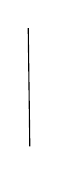
\begin{tikzpicture}\draw (0,0)--(.02,-1.5);\end{tikzpicture}}}

\uline{Cor} Si $A$ est un relèvement de W.M. \inserted{lisse} de $A_0$ lisse sur $k$, alors $H^i(\Omega^\bullet(A/W))$ ne dépend, à isom can. près, que de $A_0$.

En fait, W-M. ne prouvent ces résultats que pour des $A_0$ ``spéciales'', mais il y en a assez de celles-ci. De plus, dans leurs notes ils ne prouvent la propriété d'invariance c) que mod torsion, i.e. en tensorisant par $K$.

\deleted{\unsure{Si}} Lorsque $X_0$ est un schéma lisse quelconque sur $k$, utilisant ces résultats, W.M. définissent \inserted{dans $[\,]$} des ``faisceaux de coh.'' \deleted{$H^*(X$} $\mathcal H^*_{X_0}$ sur $X_0$, qui sont des faisceaux de $W$-modules.

Cela ne donne pas encore d'invariants

\margin{42}
